\documentclass[acmsmall, nonacm]{acmart}
\usepackage{amsmath}
\usepackage{amsfonts}
\usepackage{amssymb}
\usepackage{graphicx}
\usepackage{listings}
\usepackage{xcolor}
\usepackage{algorithm}
\usepackage{algorithmic}


\citestyle{acmauthoryear}

\title{Mixture models for misreported data}
\subtitle{Evolution of genital warts in Catalunya}
\author{Irene Agudo Zamora}
\email{1571003@uab.cat}
\author{Biel Majó i Cornet}
\email{biel.majo@uab.cat}
\author{Nestor Bravo Egea}
\email{nestor.bravo@autonoma.cat}
\author{Miguel Esteban Fernández}
\email{miguel.esteban@uab.cat}
% Define el estilo para MATLAB
\lstdefinestyle{mystyle}{
    language=R,
    backgroundcolor=\color{violet},       % Color de fondo
    basicstyle=\ttfamily\small\color{white}, % Estilo de fuente básico
    keywordstyle=\color{green}\bfseries,  % Palabras clave en azul y negrita
    commentstyle=\color{cyan}\itshape,   % Comentarios en gris e itálica
    stringstyle=\color{red},              % Cadenas en rojo
    numberstyle=\tiny\color{magenta},       % Números de línea en gris
    stepnumber=1,                        % Mostrar números de línea
    numbers=left,                        % Mostrar números a la izquierda
    numbersep=5pt,                       % Distancia entre números y código
    showspaces=false,                    % No mostrar espacios
    showstringspaces=false,              % No mostrar espacios en cadenas
    breaklines=true,                     % Romper líneas largas automáticamente
    breakatwhitespace=true,              % Romper líneas en espacios
    captionpos=b,                        % Posición de la leyenda (abajo)
    frame=single                         % Añadir un marco alrededor del código
}

\begin{document}


\maketitle

\section{Basic Concepts: Mixture Models}

A \textit{mixture model} is a type of statistical model used to represent a population composed of several subgroups or different components, each with its own probability distribution. In this context, the subgroups are not directly observed; instead, it is assumed that the observed data is a combination of these components.

For a mixture model with \( K \) components, the general probability density function is defined as:

\[
f(x) = \sum_{k=1}^{K} \pi_k f_k(x),
\]

where:
\begin{itemize}
    \item \( f(x) \) is the probability density function for the overall mixture model.
    \item \( K \) is the number of components in the model.
    \item \( \pi_k \) is the weight or proportion of component \( k \), with \( \sum_{k=1}^{K} \pi_k = 1 \).
    \item \( f_k(x) \) is the probability density function of the \( k \)-th component.
\end{itemize}

This model is useful when representing phenomena where the observed data may belong to different subpopulations (e.g., underreported vs. fully reported data), and we aim to estimate the parameters of each subpopulation without knowing in advance to which subgroup each observation belongs. The relevance of the probability density function in a mixture model lies in its ability to formally define this combination of subpopulations and, through an iterative fitting process, obtain parameter estimates that best describe the observed data.

\section{Parameter Estimation: The EM Algorithm}

To estimate the parameters of each component in a mixture model, the \textit{Expectation-Maximization} (EM) algorithm is commonly used. This is an iterative algorithm that maximizes the log-likelihood of the observed data. The process consists of two steps: the E-step and the M-step.

1. \textbf{E-Step (Expectation):} Given the current value of the parameters, the algorithm calculates the expected value of the log-likelihood of the complete data (observed and latent), based on the observed data and the current parameters. The complete-data log-likelihood function is:

    \[
    l(X, Z; \theta) = \sum_{j=1}^n \log\left(\sum_{i=1}^k I_i(z_j) f_i(x_j; \theta_i)\right),
    \]

    where:
    \begin{itemize}
        \item \( X = \{x_1, x_2, \dots, x_n\} \) are the observed data.
        \item \( Z = \{z_1, z_2, \dots, z_n\} \) represents the latent variables indicating which component each observation \( x_j \) belongs to.
        \item \( \theta = \{\theta_1, \dots, \theta_k, \omega_1, \dots, \omega_k\} \) is the set of model parameters.
        \item \( I_i(z_j) \) is an indicator variable that equals 1 if \( z_j \) corresponds to component \( i \), and 0 otherwise.
    \end{itemize}

    Since \( I_i(z_j) \) is unknown, it is replaced by its expected conditional value given \( X = x_j \) and the current parameters, denoted as \( \gamma_{i,j}^0 \) (responsibility of component \( i \) over observation \( j \)):

    \[
    E(I_i(z_j) \mid X = x_j) = P(I_i(z_j) = 1 \mid X = x_j) = \frac{f_i(x_j; \theta_i^0) \omega_i^0}{\sum_{i=1}^k f_i(x_j; \theta_i^0) \omega_i^0} = \gamma_{i,j}^0.
    \]

2. \textbf{M-Step (Maximization):} In this step, the model parameters are maximized to improve the approximate log-likelihood function:

    \[
    l(X, Z; \theta) \approx q(X, \theta) = \sum_{j=1}^n \sum_{i=1}^k \gamma_{i,j}^0 \log(f_i(x_j; \theta_i)),
    \]

    obtaining new values for the parameters \( \theta \) that increase the likelihood of the data. These parameters are updated, and the process repeats until convergence is achieved.

\section{Modeling Underreported Data}

For underreported data, the structure of a mixture model captures the probability that an observation is either fully reported or underreported. Mathematically, this model can be expressed as:

\[
Y_t = 
\begin{cases} 
X_t & \text{with probability } 1 - \omega_t \\ 
q \cdot X_t & \text{with probability } \omega_t,
\end{cases}
\]

where \( 0 < q < 1 \) represents the intensity of underreporting, and \( \omega_t \) is the probability that observation \( Y_t \) is underreported.

\section{Modeling Genital Warts Incidence in Catalonia}

In this specific context, the series \( Y_t \) of genital warts incidence is modeled as a mixture of two normal random variables, with the following probabilistic structure:

\[
Y_t = 
\begin{cases} 
Y_{1t} & \text{with probability } 1 - \omega_t, \\ 
Y_{2t} & \text{with probability } \omega_t,
\end{cases}
\]

where \( \omega_t \) is the probability of underreporting at time \( t \).

In this context:

\begin{itemize}
    \item \( Y_{1t} \) is chosen with probability \( 1 - \omega_t \), representing the case where no underreporting occurs.
    \item \( Y_{2t} \) is chosen with probability \( \omega_t \), representing the case where underreporting occurs.
\end{itemize}

\begin{itemize}
    \item \( Y_{1t} \) is a normal variable with mean \( \mu \) and variance \( \sigma^2 \), while \( Y_{2t} \) is a normal variable with mean \( q \cdot \mu \) and variance \( q^2 \cdot \sigma^2 \).
    \item \( \omega_t \) is modeled as \( \omega_t = \frac{\exp^{\alpha_0 + \alpha_1t}}{1+\exp^{\alpha_0 + \alpha_1t}} \), allowing a time-varying probability of underreporting.
    \item The mean of the first component is modeled as:

    \[
    \mu_{1,t} = \beta_0 + \beta_1 \cdot t + \beta_2 \cdot a + \beta_3 \cdot s + \beta_4 \cdot (a \ast s) + \beta_5 \cdot \sin\left(\frac{2 \pi t}{3}\right) + \beta_6 \cdot \cos\left(\frac{2 \pi t}{3}\right),
    \]

    where \( a \) is age, \( s \) is sex, and \( a \ast s \) represents the interaction between age and sex.

    \item The mean of the second component can be recovered as:

    \[
    \mu_{2,t} = q \cdot \left(\beta_0 + \beta_1 \cdot t + \beta_2 \cdot a + \beta_3 \cdot s + \beta_4 \cdot (a \ast s) + \beta_5 \cdot \sin\left(\frac{2 \pi t}{3}\right) + \beta_6 \cdot \cos\left(\frac{2 \pi t}{3}\right)\right).
    \]
\end{itemize}

This model captures both the temporal dynamics of incidence and potential underreporting in public health data, applying the mixture model to differentiate between fully reported and underreported cases of genital warts.

\section*{Log-Likelihood Function}

For the mixture model with underreported data, the log-likelihood function captures the probability of observing the data \( Y_t \) given the components \( Y_{1t} \) and \( Y_{2t} \) with respective probabilities \( 1 - \omega_t \) and \( \omega_t \). In this case:

\[
Y_t = 
\begin{cases} 
Y_{1t} & \text{with probability } 1 - \omega_t, \\ 
Y_{2t} & \text{with probability } \omega_t,
\end{cases}
\]

where \( Y_{1t} \sim \mathcal{N}(\mu, \sigma^2) \) represents non-underreported data and \( Y_{2t} \sim \mathcal{N}(q \cdot \mu, q^2 \cdot \sigma^2) \) represents underreported data. Let \( \{Y_t\}_{t=1}^T \) denote the set of observed data.

The log-likelihood function \( \ell(\theta) \), where \( \theta = (\mu, \sigma^2, q, \alpha_0, \alpha_1) \) (assuming \( \omega_t \) is modeled as a logistic function \( \logit(\omega_t) = \alpha_0 + \alpha_1 t \)), can be written as:

\[
\ell(\theta) = \sum_{t=1}^T \log \left( (1 - \omega_t) \cdot f_{Y_{1t}}(Y_t \mid \mu, \sigma^2) + \omega_t \cdot f_{Y_{2t}}(Y_t \mid q \cdot \mu, q^2 \cdot \sigma^2) \right),
\]

where:
\begin{itemize}
    \item \( f_{Y_{1t}}(Y_t \mid \mu, \sigma^2) \) is the probability density function of \( Y_{1t} \), which is \( \mathcal{N}(Y_t \mid \mu, \sigma^2) \),
    \item \( f_{Y_{2t}}(Y_t \mid q \cdot \mu, q^2 \cdot \sigma^2) \) is the probability density function of \( Y_{2t} \), which is \( \mathcal{N}(Y_t \mid q \cdot \mu, q^2 \cdot \sigma^2) \),
    \item \( \omega_t = \frac{e^{\alpha_0 + \alpha_1 t}}{1 + e^{\alpha_0 + \alpha_1 t}} \) is the probability of underreporting at time \( t \).
\end{itemize}

Expanding the density functions of the normal distributions, we obtain:

\[
\ell(\theta) = \sum_{t=1}^T \log \left( (1 - \omega_t) \cdot \frac{1}{\sqrt{2 \pi \sigma^2}} \exp\left(-\frac{(Y_t - \mu)^2}{2 \sigma^2}\right) + \omega_t \cdot \frac{1}{\sqrt{2 \pi q^2 \sigma^2}} \exp\left(-\frac{(Y_t - q \cdot \mu)^2}{2 q^2 \sigma^2}\right) \right).
\]

Here, \( T \) represents the number of observations, \( Y_t \) is the observed incidence at time \( t \), \( \mu_{1,t} \) and \( \mu_{2,t} \) are the means of the first and second components at time \( t \), \( \sigma^2 \) is the variance of the first component, and \( q^2 \sigma^2 \) is the variance of the second component. The parameters \( \theta \) are the set of parameters to estimate, specifically \( \theta = \{\alpha_0, \alpha_1, \beta_0, \beta_1, \beta_2, \beta_3, \beta_4, \beta_5, \beta_6, \sigma, \delta\} \).

This function is maximized with respect to the parameters \( \theta \) to estimate the values that best explain the observed data \( \{Y_t\}_{t=1}^T \).

\section*{Implementation of the GMM in R}
Original code from the paper has been refactored and rewritet in order to be more clear and to, in a future work, implement new features. The new code, which performes exactly the same operartion, can be seen in the attached document of the delivery.

The GMM is implemented in R. The pseudoalgorithm can be seen in Algorithm 1.
\\\\
Key points of it are the estimation of the initial parameters, which will be used to initialize the optimization process, and the estimation of the weights and the mean effect for each time point. Finaly, the algorithm reconstructs the incidence data using the posterior probabilities and the estimated value of $q$. So it is possible to compare the reconstructed data with the observed data and check how the underreported cases of genital warts are distributed over time and demographic groups.
\begin{algorithm}
    \label{al:1}
    \caption{Analysis of Incidence Data using a Mixture Model Approach}
    \begin{algorithmic}[1]
    \STATE {Initialize:} Define covariates
    \[
    \text{covars} \gets \{t, \text{age}, \text{gender}, \text{age-gender}, \sin(2\pi t / 3), \cos(2\pi t / 3)\}.
    \]
    \STATE {Estimate Initial Parameters:}
    \STATE Initialize weights $w_0 \gets 0.7$, $q_0 \gets 0.5$.
    \STATE Perform regression-based mixture model estimation:
    \[
    \text{prova} \gets \text{regmixEM}(\text{incidence}, \text{covars}, w_0, q_0, \text{initial coefficients}).
    \]
    \STATE {Fit Model:}
    \[
    \text{linmod} \gets \text{lm}(\text{incidence} \sim \text{covars}).
    \]
    \STATE {Maximum Likelihood Estimation:}
    \[
    \text{max.llh} \gets \text{nlm}(\text{log-likelihood function}, \text{prova parameters}, \text{covars}).
    \]
    \STATE Compute $q$:
    \[
    q \gets \frac{\exp(\text{max.llh.estimate}[11])}{1 + \exp(\text{max.llh.estimate}[11])}.
    \]
    \STATE {Estimate Incidence per Time Point:}
    \FOR{$i \in \text{sample size}$}
        \STATE Compute weight:
        \[
        w[i] \gets \frac{\exp(a + b \cdot t[i])}{1 + \exp(a + b \cdot t[i])}.
        \]
        \STATE Compute mean effect:
        \[
        m \gets \sum (\text{covariate weights} \cdot \text{covars}[i]).
        \]
        \STATE Estimate incidence:
        \[
        y_\text{est}[i] \gets w[i] \cdot m + (1 - w[i]) \cdot \frac{m}{q}.
        \]
    \ENDFOR
    \STATE {Posterior Probabilities:} Compute posterior probabilities for each demographic group.
    \STATE {Reconstruct incidence data:} Reconstruct incidence data using posterior probabilities and estimated $q$.
    \STATE Calculate reconstruction error.
    \STATE {Plot Results}
    \end{algorithmic}
\end{algorithm}
\newpage
\section{Results}
After executing the code, the results of the original paper \cite{Morina2021} had been replicated. The estimated values for the parameters are shown in Table \ref{tab:1}.
\begin{table}[h!]
    \centering
    \caption{Parameter estimates \label{tab:1}}
    \begin{tabular}{lll}
    \hline
    \textbf{Covariate} & \textbf{Parameter} & \textbf{Estimate (95\% CI)} \\
    \hline
     & $\alpha_0$ & 2.99 (1.77; 4.20) \\
        $t$ & $\alpha_1$ & -4.31 (-6.53; -2.09) \\
        & $\beta_0$ & 13.76 (7.11; 20.40) \\
        $t$ & $\beta_1$ & 0.36 (-12.75; 13.46) \\
        $age$ & $\beta_2$ & -13.53 (-14.13; -12.92) \\
        $sex$ & $\beta_3$ & -1.60 (-2.24; -0.95) \\
        $age \ast sex$ & $\beta_4$ & 3.25 (2.44; 4.06) \\
         & $\beta_5$ & 4.16 (0.44; 7.88) \\
         & $\beta_6$ & 0.52 (-5.59; 6.64) \\
         & $q$ & 0.75 (0.72; 0.77) \\
    \hline
    \end{tabular}
\end{table}
The reconstructed data are shown in Figure \ref{raro}.
\begin{figure}
    \centering
    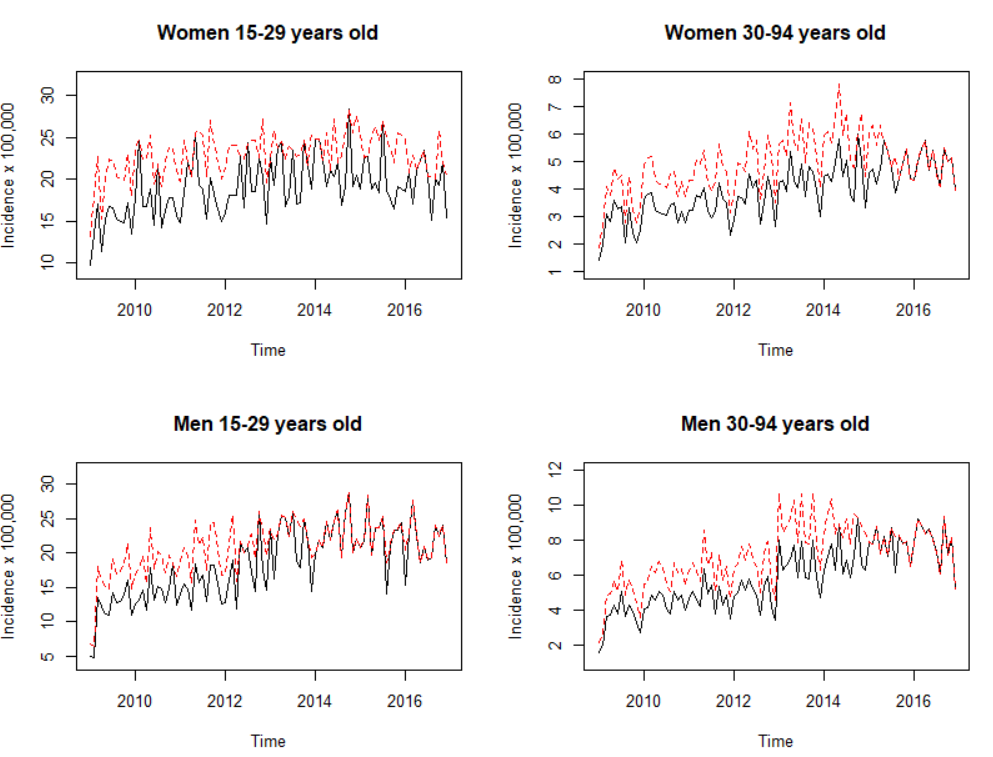
\includegraphics[width=0.8\linewidth]{raro.png}
    \caption{Registered (solid black line) and estimated underlying series (dashed red line) for each of the considered sub-populations}
    \label{raro}
\end{figure}
\\
The different residuals had also been computed and replicated shown in figure \ref{fig1} and \ref{fig2}:
\begin{figure}
    \centering
    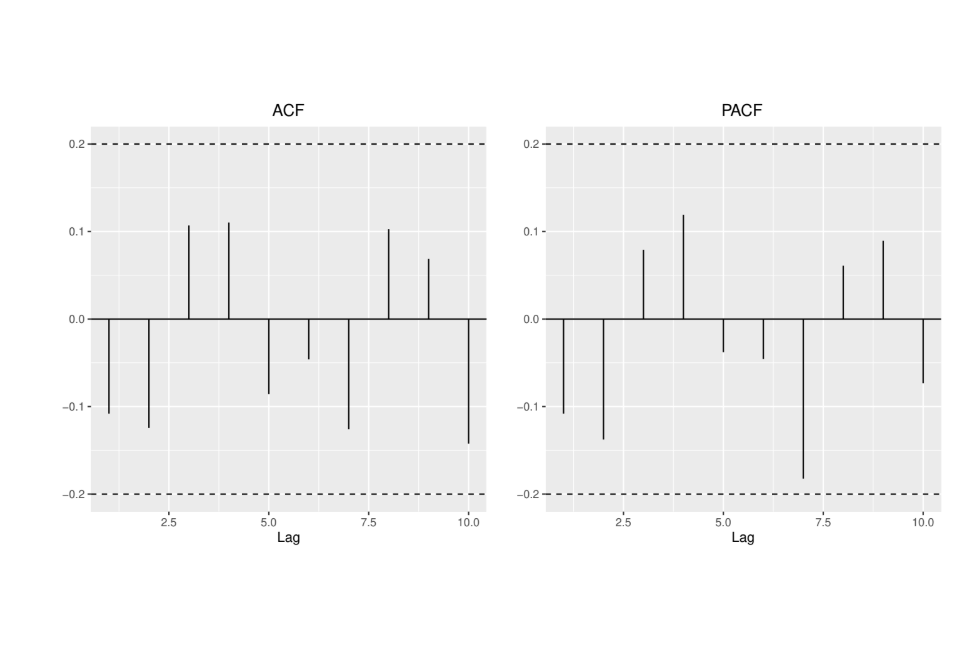
\includegraphics[width=0.8\linewidth]{fig1.png}
    \caption{Auto-correlations and partial auto-correlations of the model residuals}
    \label{fig1}
\end{figure}
\begin{figure}
    \centering
    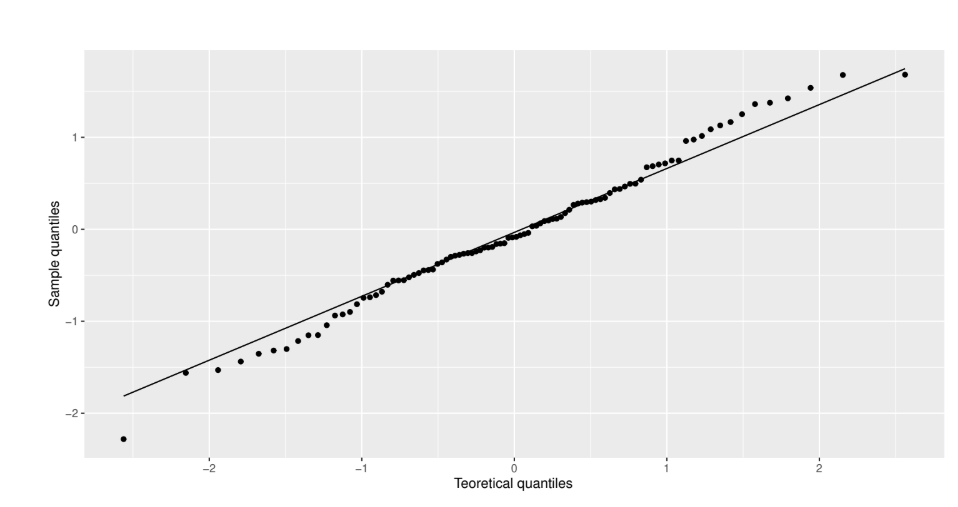
\includegraphics[width=0.8\linewidth]{fig2.png}
    \caption{Residuals qqplot}
    \label{fig2}
\end{figure}
\section{Model improvement: q time dependence}
In order to improve the model and to make it more realistic, the variable $q$ can be converted into a weight dependent on time. This will allow the model to capture the temporal dynamics of underreporting, which is a common feature in public health data. The new model will be defined as:
\[
Y_t = 
\begin{cases} 
X_t & \text{with probability } 1 - \omega_t \\ 
q_t \cdot X_t & \text{with probability } \omega_t,
\end{cases}
\]
where $q_t$ is a time-dependent weight that captures the intensity of underreporting at time $t$.

To implement this new feature, the same strategy as $w_t$ will be used. Using the logistic function, $q_t$ will be defined as:
\[
q_t = \frac{e^{\gamma_0 + \gamma_1 \cdot t}}{1 + e^{\gamma_0 + \gamma_1 \cdot t}},
\]
where $\gamma_0$ and $\gamma_1$ are the new parameters to estimate

So, it is possible to estimate the new parameters $\gamma_0$ and $\gamma_1$ using the same procedure for $w_t$ as before. In the pseudocode, we must modify the following line:
\begin{algorithm}
    \label{al:1}
    \caption{Previous q estimation}
    \begin{algorithmic}[1]
    \STATE Compute $q$:
    \[
    q \gets \frac{\exp(\text{max.llh.estimate}[11])}{1 + \exp(\text{max.llh.estimate}[11])}.
    \]
    \\
    \[(...)\]
    \STATE Estimate incidence:
        \[
        y_\text{est}[i] \gets w[i] \cdot m + (1 - w[i]) \cdot \frac{m}{q}.
        \]
    \end{algorithmic}
\end{algorithm}
By the following:
\begin{algorithm}
    \label{al:1}
    \caption{New $q_t$ time dependent estimation}
    \begin{algorithmic}[1]
    \STATE Compute $q$:
    \[
    q[i] \gets \frac{\exp(c+\text{max.llh.estimate}[11] \cdot t[i])}{1 + \exp(c+\text{max.llh.estimate}[11]\cdot t[i])}.
    \]
    \[(...)\]
    \STATE Estimate incidence:
        \[
        y_\text{est}[i] \gets w[i] \cdot m + (1 - w[i]) \cdot \frac{m}{q[i]}.
        \]
    \end{algorithmic}
\end{algorithm}
\subsection*{Results}
After this new implementations, we can recompute the results.









\section{Conclusions and future work}




\begin{thebibliography}{99}

\bibitem{Morina2021}
David Moriña, Amanda Fernández-Fontelo, Alejandra Cabaña, Pedro Puig, Laura Monfil, Maria Brotons, and Mireia Diaz.
\textit{Quantifying the under-reporting of uncorrelated longitudinal data: the genital warts example}.
\textit{BMC Medical Research Methodology}, 21(1):6, 2021.
DOI: \url{https://doi.org/10.1186/s12874-020-01188-4}.

\end{thebibliography}

\end{document}


